\documentclass[border=2pt,tikz]{standalone}
% Shared TikZ/pgfplots style for every figure in the manuscript.
\usepackage[T1]{fontenc}
\usepackage{mathpazo}
\usepackage{amsmath,amssymb}
\usepackage{tikz}
\usepackage{pgfplots}
\usepackage{pgfplotstable}
\pgfplotsset{compat=1.18}
\usetikzlibrary{arrows.meta,positioning,calc,backgrounds,fit,shapes.geometric}
\usepgfplotslibrary{fillbetween}

% --- palette: colour-blind safe, legible in greyscale -------------------
\definecolor{cHyd}{HTML}{1B6CA8}   % hydride / primary blue
\definecolor{cPro}{HTML}{C1492E}   % proton  / primary red
\definecolor{cAcc}{HTML}{7B5AA6}   % accent  / purple
\definecolor{cGold}{HTML}{B8860B}  % accent  / gold
\definecolor{cGrey}{HTML}{6E6E6E}
\definecolor{cInk}{HTML}{1A1A1A}
\definecolor{cBandR}{HTML}{C1492E}
\definecolor{cBandG}{HTML}{4F7942}

% --- base axis ----------------------------------------------------------
\pgfplotsset{
  icig/.style={
    width=68mm, height=52mm,
    scale only axis,
    axis line style={cInk, line width=0.45pt},
    tick style={cInk, line width=0.4pt},
    tick align=outside, tick pos=left,
    label style={font=\small, color=cInk},
    tick label style={font=\footnotesize, color=cInk},
    title style={font=\small\bfseries, color=cInk, align=left},
    legend cell align=left,
    legend style={draw=none, fill=none, font=\scriptsize,
                  inner sep=1pt, row sep=0.5pt},
    grid=both,
    major grid style={cGrey!22, line width=0.28pt},
    minor grid style={cGrey!12, line width=0.2pt},
  },
  % marker shorthands
  ptA/.style={mark=*, mark size=1.7pt, thick,
              mark options={fill=cHyd, draw=white, line width=0.4pt}},
  ptB/.style={mark=*, mark size=1.7pt, thick,
              mark options={fill=cPro, draw=white, line width=0.4pt}},
  hollowB/.style={mark=o, mark size=1.7pt, thick,
              mark options={draw=cPro, line width=0.7pt}},
}

% panel tag, e.g. \panel{a}
\newcommand{\panel}[1]{\textbf{(\textsf{#1})}}

% --- shared notation, matching the manuscript preamble ----------------
\newcommand{\KHT}{K_{\mathrm{HT}}}
\newcommand{\KDT}{K_{\mathrm{DT}}}
\newcommand{\gSC}{\gamma_{\mathrm{SC}}}
\newcommand{\Fz}{F_{0}}

\begin{document}
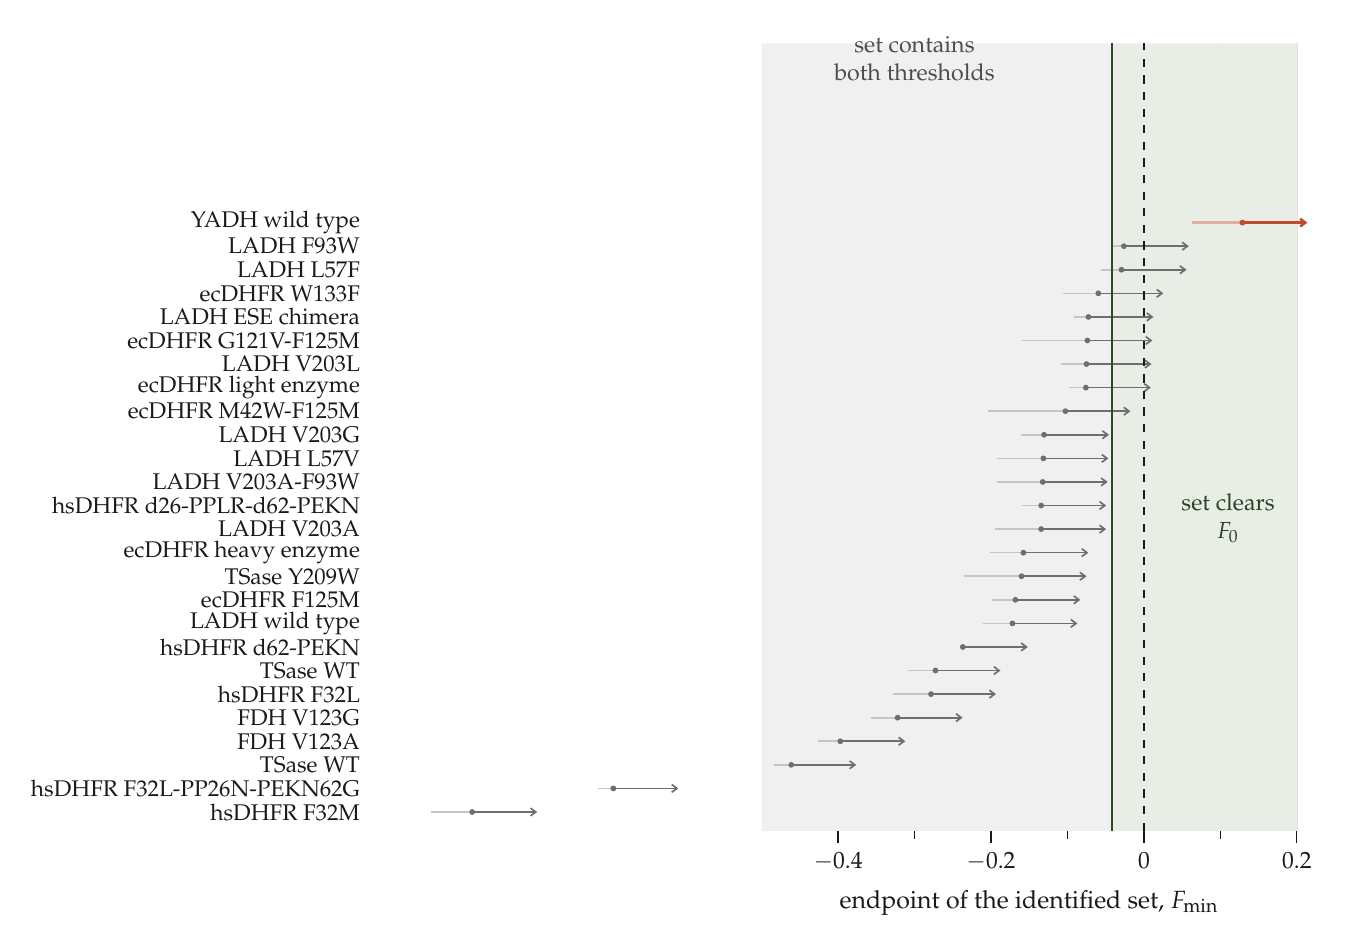
\begin{tikzpicture}
% Double-column figure, ~130 mm wide and ~113 mm tall, drawn at final size so no rescaling
% occurs in the manuscript and the type sizes below are the ones the reader sees.
% Until 2026-09-15 it was drawn single-column at 87 mm with 6.2 pt row labels,
% which a review measured as too small for print; double-column figures of
% 300-504 pt are standard.  The axis is cut at -0.50; the two systems below it carry their
% endpoints in the row label.  |F0| spans ~3.5 mm here, so the magnified inset
% used by the earlier two-column version is unnecessary.
\pgfplotsset{
  asym/.style={icig, scale only axis,
    label style={font=\fontsize{9}{10.8}\selectfont, color=cInk},
    tick label style={font=\fontsize{8.5}{10.2}\selectfont, color=cInk}},
}
\tikzset{
  rowlab/.style={font=\fontsize{8.2}{9.6}\selectfont, color=cInk,
                 anchor=east, inner sep=1.2pt},
  annc/.style={font=\fontsize{8.4}{10}\selectfont, color=cInk, align=center},
}

\begin{axis}[asym, name=A, width=68mm, height=100mm,
  xmin=-0.50, xmax=0.20, ymin=0.2, ymax=33.6,
  xlabel={endpoint of the identified set, $F_{\min}$},
  ytick=\empty, ymajorgrids=false,
  y axis line style={draw=none}, ytick style={draw=none},
  xtick={-0.4,-0.2,0,0.2}, minor x tick num=1,
  xticklabel style={/pgf/number format/.cd, fixed, precision=1, /tikz/.cd},
  clip=false]

  % left of F0 the set contains both thresholds; right of it the set clears F0
  \addplot[draw=none, fill=cGrey!10] coordinates
    {(-0.50,0.2) (-0.042086,0.2) (-0.042086,33.6) (-0.50,33.6)} \closedcycle;
  \addplot[draw=none, fill=cBandG!13] coordinates
    {(-0.042086,0.2) (0.20,0.2) (0.20,33.6) (-0.042086,33.6)} \closedcycle;

  % generated by export_fig_asym.py -- do not edit
\draw[cGrey, line width=0.6pt, -{Straight Barb[length=1.9pt,width=2.8pt]}] (axis cs:-0.87824,1) -- (axis cs:-0.79324,1);
\draw[cGrey!40, line width=0.6pt] (axis cs:-0.93230,1) -- (axis cs:-0.87824,1);
\fill[cGrey] (axis cs:-0.87824,1) circle (1.05pt);
\node[rowlab] at (axis cs:-1.02,1) {hsDHFR F32M};
\draw[cGrey, line width=0.6pt, -{Straight Barb[length=1.9pt,width=2.8pt]}] (axis cs:-0.69370,2) -- (axis cs:-0.60870,2);
\draw[cGrey!40, line width=0.6pt] (axis cs:-0.71315,2) -- (axis cs:-0.69370,2);
\fill[cGrey] (axis cs:-0.69370,2) circle (1.05pt);
\node[rowlab] at (axis cs:-1.02,2) {hsDHFR F32L-PP26N-PEKN62G};
\draw[cGrey, line width=0.6pt, -{Straight Barb[length=1.9pt,width=2.8pt]}] (axis cs:-0.46107,3) -- (axis cs:-0.37607,3);
\draw[cGrey!40, line width=0.6pt] (axis cs:-0.48417,3) -- (axis cs:-0.46107,3);
\fill[cGrey] (axis cs:-0.46107,3) circle (1.05pt);
\node[rowlab] at (axis cs:-1.02,3) {TSase WT};
\draw[cGrey, line width=0.6pt, -{Straight Barb[length=1.9pt,width=2.8pt]}] (axis cs:-0.39694,4) -- (axis cs:-0.31194,4);
\draw[cGrey!40, line width=0.6pt] (axis cs:-0.42586,4) -- (axis cs:-0.39694,4);
\fill[cGrey] (axis cs:-0.39694,4) circle (1.05pt);
\node[rowlab] at (axis cs:-1.02,4) {FDH V123A};
\draw[cGrey, line width=0.6pt, -{Straight Barb[length=1.9pt,width=2.8pt]}] (axis cs:-0.32202,5) -- (axis cs:-0.23702,5);
\draw[cGrey!40, line width=0.6pt] (axis cs:-0.35722,5) -- (axis cs:-0.32202,5);
\fill[cGrey] (axis cs:-0.32202,5) circle (1.05pt);
\node[rowlab] at (axis cs:-1.02,5) {FDH V123G};
\draw[cGrey, line width=0.6pt, -{Straight Barb[length=1.9pt,width=2.8pt]}] (axis cs:-0.27838,6) -- (axis cs:-0.19338,6);
\draw[cGrey!40, line width=0.6pt] (axis cs:-0.32864,6) -- (axis cs:-0.27838,6);
\fill[cGrey] (axis cs:-0.27838,6) circle (1.05pt);
\node[rowlab] at (axis cs:-1.02,6) {hsDHFR F32L};
\draw[cGrey, line width=0.6pt, -{Straight Barb[length=1.9pt,width=2.8pt]}] (axis cs:-0.27255,7) -- (axis cs:-0.18755,7);
\draw[cGrey!40, line width=0.6pt] (axis cs:-0.30802,7) -- (axis cs:-0.27255,7);
\fill[cGrey] (axis cs:-0.27255,7) circle (1.05pt);
\node[rowlab] at (axis cs:-1.02,7) {TSase WT};
\draw[cGrey, line width=0.6pt, -{Straight Barb[length=1.9pt,width=2.8pt]}] (axis cs:-0.23681,8) -- (axis cs:-0.15181,8);
\draw[cGrey!40, line width=0.6pt] (axis cs:-0.23835,8) -- (axis cs:-0.23681,8);
\fill[cGrey] (axis cs:-0.23681,8) circle (1.05pt);
\node[rowlab] at (axis cs:-1.02,8) {hsDHFR d62-PEKN};
\draw[cGrey, line width=0.6pt, -{Straight Barb[length=1.9pt,width=2.8pt]}] (axis cs:-0.17192,9) -- (axis cs:-0.08692,9);
\draw[cGrey!40, line width=0.6pt] (axis cs:-0.21017,9) -- (axis cs:-0.17192,9);
\fill[cGrey] (axis cs:-0.17192,9) circle (1.05pt);
\node[rowlab] at (axis cs:-1.02,9) {LADH wild type};
\draw[cGrey, line width=0.6pt, -{Straight Barb[length=1.9pt,width=2.8pt]}] (axis cs:-0.16805,10) -- (axis cs:-0.08305,10);
\draw[cGrey!40, line width=0.6pt] (axis cs:-0.19820,10) -- (axis cs:-0.16805,10);
\fill[cGrey] (axis cs:-0.16805,10) circle (1.05pt);
\node[rowlab] at (axis cs:-1.02,10) {ecDHFR F125M};
\draw[cGrey, line width=0.6pt, -{Straight Barb[length=1.9pt,width=2.8pt]}] (axis cs:-0.16004,11) -- (axis cs:-0.07504,11);
\draw[cGrey!40, line width=0.6pt] (axis cs:-0.23544,11) -- (axis cs:-0.16004,11);
\fill[cGrey] (axis cs:-0.16004,11) circle (1.05pt);
\node[rowlab] at (axis cs:-1.02,11) {TSase Y209W};
\draw[cGrey, line width=0.6pt, -{Straight Barb[length=1.9pt,width=2.8pt]}] (axis cs:-0.15761,12) -- (axis cs:-0.07261,12);
\draw[cGrey!40, line width=0.6pt] (axis cs:-0.20112,12) -- (axis cs:-0.15761,12);
\fill[cGrey] (axis cs:-0.15761,12) circle (1.05pt);
\node[rowlab] at (axis cs:-1.02,12) {ecDHFR heavy enzyme};
\draw[cGrey, line width=0.6pt, -{Straight Barb[length=1.9pt,width=2.8pt]}] (axis cs:-0.13442,13) -- (axis cs:-0.04942,13);
\draw[cGrey!40, line width=0.6pt] (axis cs:-0.19459,13) -- (axis cs:-0.13442,13);
\fill[cGrey] (axis cs:-0.13442,13) circle (1.05pt);
\node[rowlab] at (axis cs:-1.02,13) {LADH V203A};
\draw[cGrey, line width=0.6pt, -{Straight Barb[length=1.9pt,width=2.8pt]}] (axis cs:-0.13435,14) -- (axis cs:-0.04935,14);
\draw[cGrey!40, line width=0.6pt] (axis cs:-0.15982,14) -- (axis cs:-0.13435,14);
\fill[cGrey] (axis cs:-0.13435,14) circle (1.05pt);
\node[rowlab] at (axis cs:-1.02,14) {hsDHFR d26-PPLR-d62-PEKN};
\draw[cGrey, line width=0.6pt, -{Straight Barb[length=1.9pt,width=2.8pt]}] (axis cs:-0.13236,15) -- (axis cs:-0.04736,15);
\draw[cGrey!40, line width=0.6pt] (axis cs:-0.19147,15) -- (axis cs:-0.13236,15);
\fill[cGrey] (axis cs:-0.13236,15) circle (1.05pt);
\node[rowlab] at (axis cs:-1.02,15) {LADH V203A-F93W};
\draw[cGrey, line width=0.6pt, -{Straight Barb[length=1.9pt,width=2.8pt]}] (axis cs:-0.13146,16) -- (axis cs:-0.04646,16);
\draw[cGrey!40, line width=0.6pt] (axis cs:-0.19263,16) -- (axis cs:-0.13146,16);
\fill[cGrey] (axis cs:-0.13146,16) circle (1.05pt);
\node[rowlab] at (axis cs:-1.02,16) {LADH L57V};
\draw[cGrey, line width=0.6pt, -{Straight Barb[length=1.9pt,width=2.8pt]}] (axis cs:-0.13059,17) -- (axis cs:-0.04559,17);
\draw[cGrey!40, line width=0.6pt] (axis cs:-0.16031,17) -- (axis cs:-0.13059,17);
\fill[cGrey] (axis cs:-0.13059,17) circle (1.05pt);
\node[rowlab] at (axis cs:-1.02,17) {LADH V203G};
\draw[cGrey, line width=0.6pt, -{Straight Barb[length=1.9pt,width=2.8pt]}] (axis cs:-0.10265,18) -- (axis cs:-0.01765,18);
\draw[cGrey!40, line width=0.6pt] (axis cs:-0.20413,18) -- (axis cs:-0.10265,18);
\fill[cGrey] (axis cs:-0.10265,18) circle (1.05pt);
\node[rowlab] at (axis cs:-1.02,18) {ecDHFR M42W-F125M};
\draw[cGrey, line width=0.6pt, -{Straight Barb[length=1.9pt,width=2.8pt]}] (axis cs:-0.07594,19) -- (axis cs:0.00906,19);
\draw[cGrey!40, line width=0.6pt] (axis cs:-0.09749,19) -- (axis cs:-0.07594,19);
\fill[cGrey] (axis cs:-0.07594,19) circle (1.05pt);
\node[rowlab] at (axis cs:-1.02,19) {ecDHFR light enzyme};
\draw[cGrey, line width=0.6pt, -{Straight Barb[length=1.9pt,width=2.8pt]}] (axis cs:-0.07513,20) -- (axis cs:0.00987,20);
\draw[cGrey!40, line width=0.6pt] (axis cs:-0.10878,20) -- (axis cs:-0.07513,20);
\fill[cGrey] (axis cs:-0.07513,20) circle (1.05pt);
\node[rowlab] at (axis cs:-1.02,20) {LADH V203L};
\draw[cGrey, line width=0.6pt, -{Straight Barb[length=1.9pt,width=2.8pt]}] (axis cs:-0.07395,21) -- (axis cs:0.01105,21);
\draw[cGrey!40, line width=0.6pt] (axis cs:-0.15938,21) -- (axis cs:-0.07395,21);
\fill[cGrey] (axis cs:-0.07395,21) circle (1.05pt);
\node[rowlab] at (axis cs:-1.02,21) {ecDHFR G121V-F125M};
\draw[cGrey, line width=0.6pt, -{Straight Barb[length=1.9pt,width=2.8pt]}] (axis cs:-0.07254,22) -- (axis cs:0.01246,22);
\draw[cGrey!40, line width=0.6pt] (axis cs:-0.09184,22) -- (axis cs:-0.07254,22);
\fill[cGrey] (axis cs:-0.07254,22) circle (1.05pt);
\node[rowlab] at (axis cs:-1.02,22) {LADH ESE chimera};
\draw[cGrey, line width=0.6pt, -{Straight Barb[length=1.9pt,width=2.8pt]}] (axis cs:-0.05962,23) -- (axis cs:0.02538,23);
\draw[cGrey!40, line width=0.6pt] (axis cs:-0.10547,23) -- (axis cs:-0.05962,23);
\fill[cGrey] (axis cs:-0.05962,23) circle (1.05pt);
\node[rowlab] at (axis cs:-1.02,23) {ecDHFR W133F};
\draw[cGrey, line width=0.6pt, -{Straight Barb[length=1.9pt,width=2.8pt]}] (axis cs:-0.02931,24) -- (axis cs:0.05569,24);
\draw[cGrey!40, line width=0.6pt] (axis cs:-0.05574,24) -- (axis cs:-0.02931,24);
\fill[cGrey] (axis cs:-0.02931,24) circle (1.05pt);
\node[rowlab] at (axis cs:-1.02,24) {LADH L57F};
\draw[cGrey, line width=0.6pt, -{Straight Barb[length=1.9pt,width=2.8pt]}] (axis cs:-0.02629,25) -- (axis cs:0.05871,25);
\draw[cGrey!40, line width=0.6pt] (axis cs:-0.04277,25) -- (axis cs:-0.02629,25);
\fill[cGrey] (axis cs:-0.02629,25) circle (1.05pt);
\node[rowlab] at (axis cs:-1.02,25) {LADH F93W};
\draw[cPro, line width=0.9pt, -{Straight Barb[length=1.9pt,width=2.8pt]}] (axis cs:0.12873,26) -- (axis cs:0.21373,26);
\draw[cPro!45, line width=0.9pt] (axis cs:0.06302,26) -- (axis cs:0.12873,26);
\fill[cPro] (axis cs:0.12873,26) circle (1.05pt);
\node[rowlab] at (axis cs:-1.02,26) {YADH wild type};


  \draw[cBandG!60!black, line width=0.6pt] (axis cs:-0.042086,0.2) --
       (axis cs:-0.042086,33.6);
  \draw[cInk, line width=0.5pt, dashed] (axis cs:0,0.2) -- (axis cs:0,33.6);

  % Short forms: the narrower axis leaves no room for the fuller wording, and
  % the caption carries it.  The red key is dropped for the same reason.
  \node[annc, anchor=south, color=cGrey!70!black] at (axis cs:-0.30,31.6)
    {set contains\\both thresholds};
  % Placed below the three rows that reach past F0, not above them: at the top
  % it covered the yeast ray, the one row the region exists to show.
  \node[annc, anchor=south, color=cBandG!55!black] at (axis cs:0.110,12.0)
    {set clears\\$\Fz$};
\end{axis}
\end{tikzpicture}
\end{document}
